\section{Comparative Evaluation Protocol}

To move beyond narrative comparison, the review includes a compact benchmark design centered on a single mixed study area. The current pilot region is the Wuhan East Lake and Tangxun Lake corridor in China, selected because it combines urban fabric, water bodies, cropland, and vegetation within a limited spatial extent. This diversity makes it possible to study several downstream tasks without switching datasets or geographic context.

\subsection{Pilot study area}

The Wuhan pilot is not intended to replace global benchmarks. Its role is to provide one controlled, mixed-landscape setting in which multiple embedding families can be compared under shared spatial context, labels, and extraction windows.

\subsection{Benchmark tasks and protocol}

The first benchmark pass uses three task families:

\begin{enumerate}[leftmargin=1.4em]
  \item tile classification over coarse WorldCover classes;
  \item water segmentation with JRC Global Surface Water or Dynamic World labels;
  \item tile-level fraction regression for built-up or vegetation proportion.
\end{enumerate}

All models use the same tile centroids, train/validation/test split, and lightweight probe heads. Annual product models are evaluated at the nearest available year, while on-the-fly models use a common Sentinel-2 temporal window. Encoder weights remain frozen in the first pass so that the benchmark measures representation quality rather than fine-tuning capacity.

\begin{figure}[t]
  \centering
  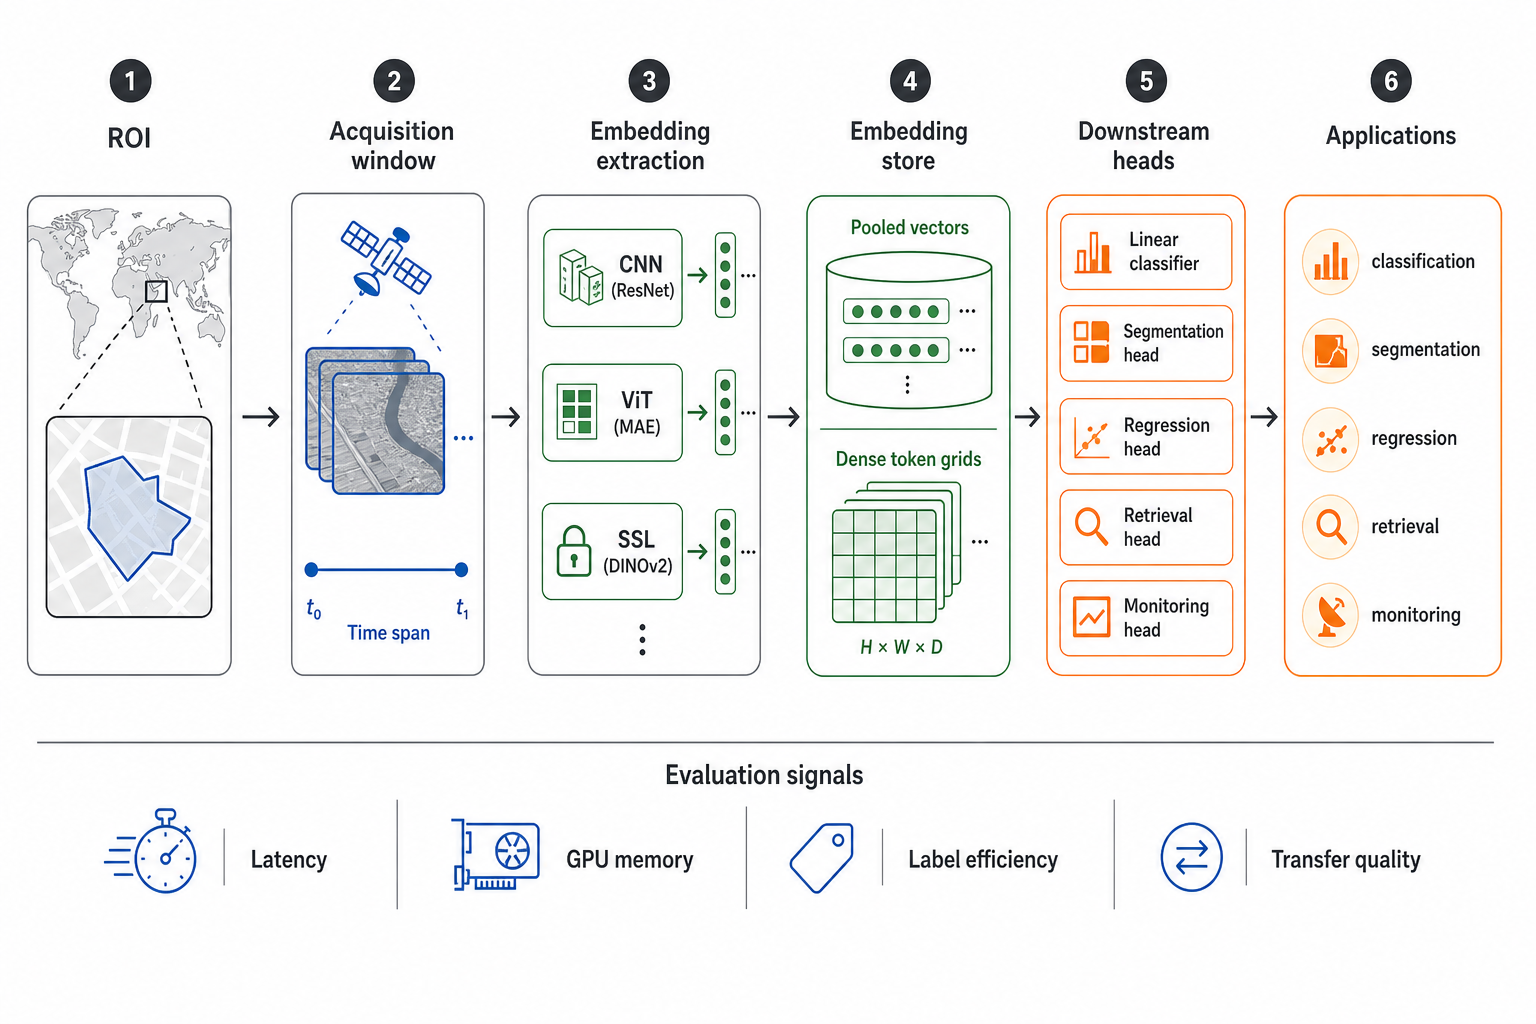
\includegraphics[width=\textwidth]{fig02_application_pipeline_gptimage2_20260502.png}
  \caption{Application-oriented benchmark pipeline. A shared region of interest is converted into a unified embedding extraction workflow, lightweight probe heads, and downstream evaluation targets spanning classification, segmentation, regression, and retrieval.}
  \label{fig:application-pipeline}
\end{figure}

\subsection{Why a small-area protocol is still informative}

A compact benchmark cannot replace global evaluation, but it can reveal the practical trade-offs that matter most during model selection. Specifically, it highlights scale mismatch, the effect of temporal summarization, and the difference between pooled-only and dense-capable representations. It also lowers the cost of iteration, making it easier to add new models or new downstream heads as the repository evolves. Figure~\ref{fig:application-pipeline} shows the intended experiment flow that will populate the comparison tables in the next draft.

\subsection{Expected outputs}

The benchmark should produce one table that combines quality and runtime, a quality-versus-latency figure, and a family-level transfer summary. These artifacts will directly support the application section of the survey and can also feed the interactive explorer described in Section~\ref{sec:system-layer}.

\subsection{First executed pilot}

The first executed pass now uses the Wuhan East Lake ROI already defined in this survey workspace, but with a deliberately conservative task setup chosen to ensure balanced labels and fast iteration. Instead of forcing a sparse 6-class classification problem in a compact urban-water corridor, the executed pilot collapses the label space into three dominant classes: \emph{water}, \emph{green}, and \emph{built}. A regular \(10 \times 10\) candidate grid with 500\,m square buffers was generated inside the ROI, ESA WorldCover 2021 and JRC Global Surface Water were queried through Google Earth Engine, and 15 tiles were selected with a dominance threshold of 0.5, yielding a perfectly balanced subset of 5 tiles per class. The same tiles were then used for tile-level built fraction, green fraction, and water fraction regression.

The first model panel covers one precomputed product model (GSE), one vision-language model (RemoteCLIP), one masked autoencoder model (SatMAE++ S2-10B), one multimodal generalist encoder (Galileo), one domain-specialized temporal model (AgriFM), and one coarse-resolution precomputed product (Copernicus). Table~\ref{tab:wuhan-pilot-results} summarizes the initial results. Two observations are already useful for the review. First, several families can separate the 3-class pilot almost perfectly under frozen linear probing, suggesting that even a small-area benchmark can expose strong transfer behavior quickly. Second, deployment constraints matter as much as accuracy: Copernicus failed not because of a broken implementation, but because its 0.25\(^\circ\) native embedding pixel is fundamentally mismatched to a 500\,m local ROI. This is exactly the kind of scale-and-deployment issue that an embedding-centered review should make visible.

\begin{table*}[t]
\centering
\caption{First executed Wuhan pilot benchmark on a balanced 15-tile subset (5 water, 5 green, 5 built). The pilot uses 500\,m square buffers, frozen pooled embeddings, 3-class dominant land-cover classification, and tile-level fraction regression.}
\label{tab:wuhan-pilot-results}
\small
\begin{tabular}{lcccccc}
\toprule
Model & Status & Macro F1 & Built RMSE & Water RMSE & Time (s) & Peak GPU MB \\
\midrule
GSE & pass & 1.000 & 0.061 & 0.348 & 35.6 & 0.0 \\
SatMAE++ S2-10B & pass & 1.000 & 0.083 & 0.264 & 36.9 & 1353.8 \\
Galileo & pass & 1.000 & 0.161 & 0.305 & 87.6 & 277.3 \\
AgriFM & pass & 1.000 & 0.238 & 0.836 & 88.7 & 591.1 \\
RemoteCLIP & pass & 0.852 & 0.187 & 0.300 & 44.6 & 602.6 \\
Copernicus & fail & --- & --- & --- & --- & --- \\
\bottomrule
\end{tabular}
\end{table*}

